% ------------------------------------------------------------------------------
% TYPO3 CMS 7.1 - What's New (Serbian Version)
%
% @author	Michael Schams <schams.net>
% @license	Creative Commons BY-NC-SA 3.0
% @link		http://typo3.org/download/release-notes/whats-new/
% @language	Serbian
% ------------------------------------------------------------------------------
% LTXE-CHAPTER-UID:		e7264f0e-3f82290d-94c50cda-fb2d8e66
% LTXE-CHAPTER-NAME:	Backend User Interface
% ------------------------------------------------------------------------------

\section{Administratorski interfejs}
\begin{frame}[fragile]
	\frametitle{Administratorski interfejs}

	\begin{center}\huge{Poglavlje  1:}\end{center}
	\begin{center}\huge{\color{typo3darkgrey}\textbf{Administratorski interfejs}}\end{center}

\end{frame}

% ------------------------------------------------------------------------------
% LTXE-SLIDE-START
% LTXE-SLIDE-UID:		6663b1e8-f68c0ade-dec8bc6c-d4ac55ae
% LTXE-SLIDE-ORIGIN:	d5fddde9-b3ee31c0-f0509300-40a2928e English
% LTXE-SLIDE-TITLE:		Date/Time Picker
% LTXE-SLIDE-REFERENCE:	Breaking-62925-RemoveExtJsDateTimePicker.rst
% ------------------------------------------------------------------------------

\begin{frame}[fragile]
	\frametitle{Administratorski interfejs}
	\framesubtitle{Pogledaj i oseti: Date/Time Picker}

	Date/Time Picker je zamenjen sa Bootstrap-ovom alternativom
	\begin{figure}
		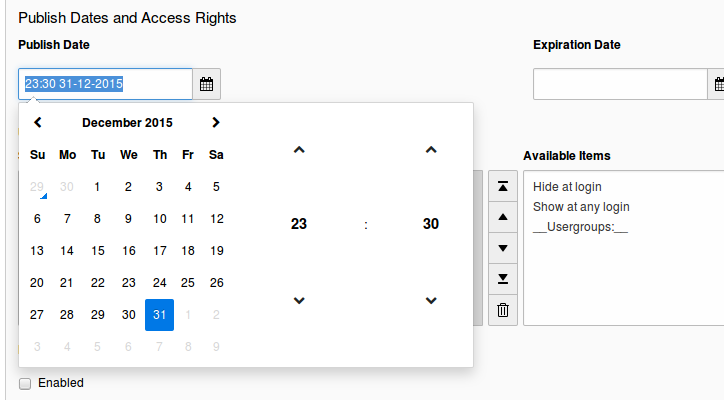
\includegraphics[width=0.75\linewidth]{BackendUserInterface/be-datepicker.png}
	\end{figure}

\end{frame}

% ------------------------------------------------------------------------------
% LTXE-SLIDE-START
% LTXE-SLIDE-UID:		827ead8c-28d29bd5-7e456f40-8b4c817c
% LTXE-SLIDE-ORIGIN:	1c391eec-dfb1dfa6-f783ae7a-d0b214ae English
% LTXE-SLIDE-TITLE:		Functions Module
% LTXE-SLIDE-REFERENCE:	Breaking-63310-Wizard-Modules-Moved.rst
% ------------------------------------------------------------------------------

\begin{frame}[fragile]
	\frametitle{Administratorski interfejs}
	\framesubtitle{Pogledaj i oseti: Functions modul}

	Napravi Strane ("Create Pages") i sortiraj strane ("Sort Pages") premesten je u \texttt{Web => Functions}\newline
	\smaller (u TYPO3 CMS < 7.1, ove opcije su se nalazile pod "\texttt{Web => Functions => Wizards}")

	\begin{figure}
		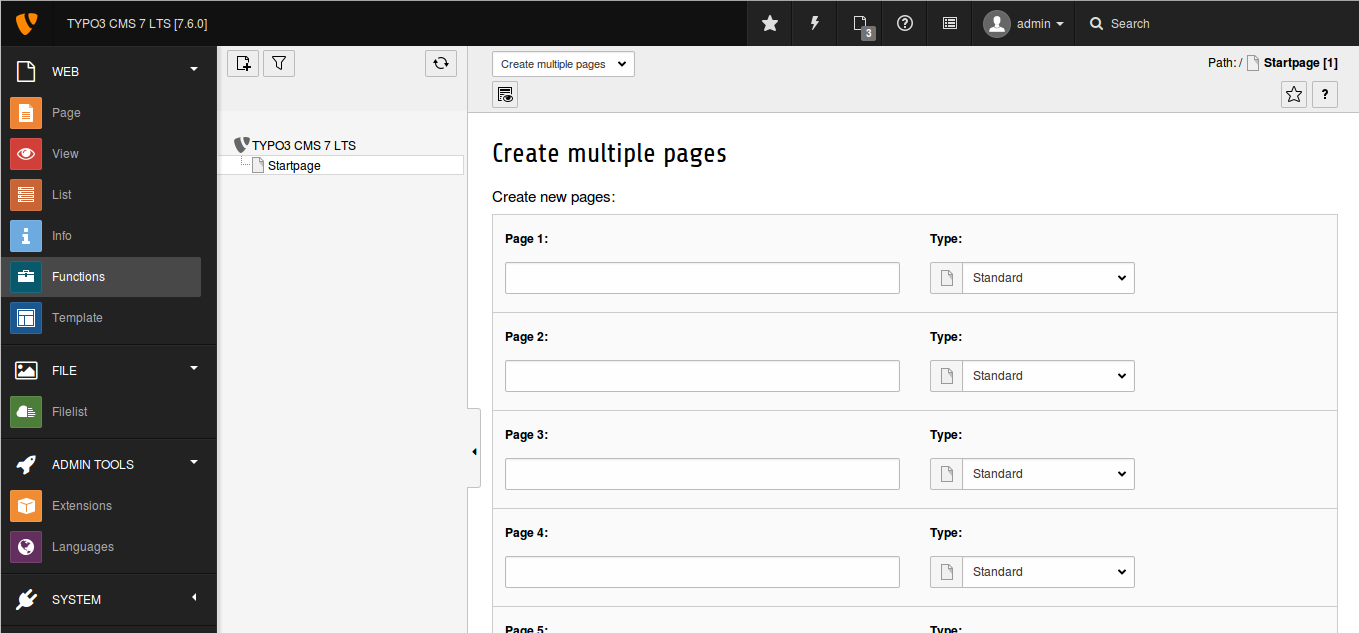
\includegraphics[width=0.80\linewidth]{BackendUserInterface/be-functions.png}
	\end{figure}


\end{frame}

% ------------------------------------------------------------------------------
% LTXE-SLIDE-START
% LTXE-SLIDE-UID:		8960cc6c-d209df1e-adf674d8-21851602
% LTXE-SLIDE-ORIGIN:	dd127630-5ccc729a-835e5836-e8796962 English
% LTXE-SLIDE-TITLE:		Access Module: Leave Unchaged
% LTXE-SLIDE-REFERENCE:	Feature-15619-LeaveUnchagedInAccessModule.rst
% ------------------------------------------------------------------------------

\begin{frame}[fragile]
	\frametitle{Administratorski interfejs}
	\framesubtitle{Pogledaj i oseti: Access modul}

	Modul \texttt{Web => Access} dozvoljava da vlasnik/grupa ostanu nepromenjeni\newline
	nakon menjanja permisija

	\begin{figure}
		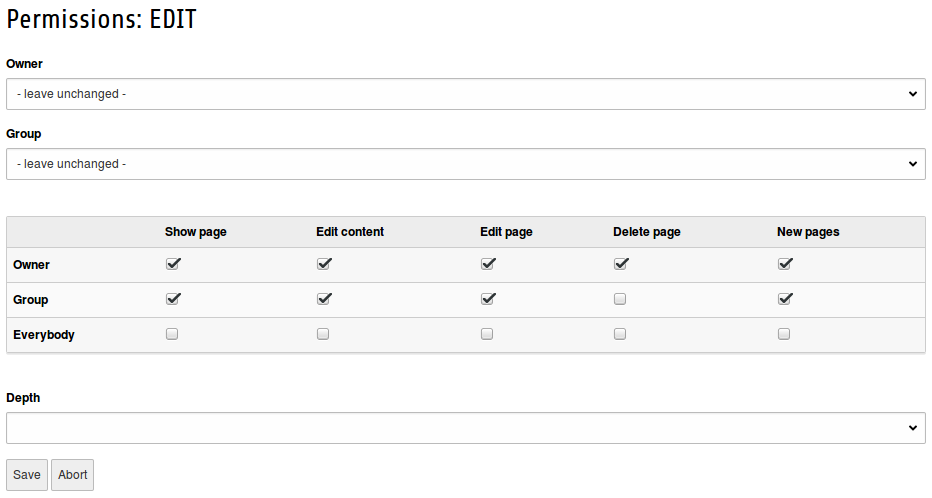
\includegraphics[width=0.75\linewidth]{BackendUserInterface/be-access.png}
	\end{figure}

\end{frame}

% ------------------------------------------------------------------------------
% LTXE-SLIDE-START
% LTXE-SLIDE-UID:		2ab8d8ce-70af5652-1da02dac-27fb0f6e
% LTXE-SLIDE-ORIGIN:	eb6cc867-e4f5d0d3-ea06672c-7ccdf227 English
% LTXE-SLIDE-TITLE:		Icons in List Module
% LTXE-SLIDE-REFERENCE:	Feature-63207-SplitActionButtonsIntoGroups.rst
% ------------------------------------------------------------------------------

\begin{frame}[fragile]
	\frametitle{Administratorski interfejs}
	\framesubtitle{Pogledaj i oseti: Ikonice u list modulu}

	Ikonice ("akcioni dugmici") podeljene su u dve grupe \newline
	\smaller (glavne akcije (read, update, delete), pracene sekundarnim akcijama)

	\begin{figure}
		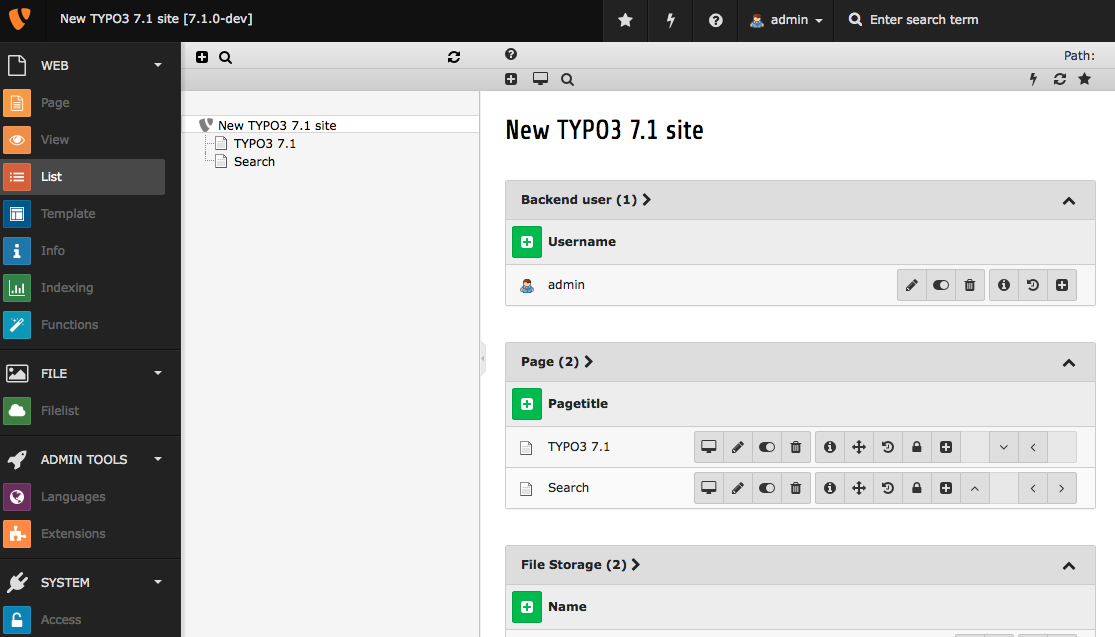
\includegraphics[width=0.75\linewidth]{BackendUserInterface/be-icons.png}
	\end{figure}

\end{frame}

% ------------------------------------------------------------------------------
